\documentclass{article}
\usepackage[spanish,es-nodecimaldot]{babel}
\usepackage[utf8]{inputenc}
\usepackage[letterpaper,top=2.5cm,bottom=2.5cm,left=2.5cm,right=2.5cm,marginparwidth=1.75cm]{geometry}

% Paquetes matemáticos y gráficos
\usepackage{amsmath}
\usepackage{amssymb}
\usepackage{graphicx}
\usepackage[colorlinks=true, allcolors=blue]{hyperref}
\usepackage{fancyhdr}
\usepackage{multicol}
\usepackage{float}
\usepackage{array}
\usepackage{longtable}
\usepackage{booktabs}
\usepackage{listings}
\usepackage{xcolor}

% Configuración para listados de código con soporte de caracteres en español
\lstset{
    basicstyle=\ttfamily\scriptsize,
    breaklines=true,
    frame=single,
    backgroundcolor=\color{gray!8},
    keywordstyle=\color{blue}\bfseries,
    commentstyle=\color{green!50!black}\itshape,
    stringstyle=\color{red!70!black},
    numbers=left,
    numberstyle=\tiny\color{gray},
    numbersep=5pt,
    tabsize=4,
    showspaces=false,
    showstringspaces=false,
    literate=
        {á}{{\'a}}1 {é}{{\'e}}1 {í}{{\'i}}1 {ó}{{\'o}}1 {ú}{{\'u}}1
        {Á}{{\'A}}1 {É}{{\'E}}1 {Í}{{\'I}}1 {Ó}{{\'O}}1 {Ú}{{\'U}}1
        {ñ}{{\~n}}1 {Ñ}{{\~N}}1 {¿}{{?`}}1 {¡}{{!`}}1
}

\pagestyle{fancy}
\fancyhf{}
\setlength{\headheight}{65pt}

% Encabezado institucional UTA / FISEI
\fancyhead[C]{%
    \begin{minipage}[c]{2.5cm}
        \centering
        
\includegraphics[width=2.0cm]{imagenes/uta.png}
    \end{minipage}%
    \hfill
    \begin{minipage}[c]{11cm}
        \centering
        \small \textbf{UNIVERSIDAD TÉCNICA DE AMBATO} \\[0.1cm]
        \scriptsize \textit{FACULTAD DE INGENIERÍA EN SISTEMAS ELECTRÓNICA E INDUSTRIAL} \\[0.1cm]
        \scriptsize \textbf{CARRERA DE SOFTWARE} \\[0.1cm]
        \scriptsize \textbf{CICLO ACADÉMICO: JULIO – DICIEMBRE 2026}
    \end{minipage}%
    \hfill
    \begin{minipage}[c]{2.5cm}
        \centering
        
\includegraphics[width=2.0cm]{imagenes/fisei.png}
    \end{minipage}%
}
\fancyfoot[C]{\thepage}

\begin{document}

\begin{center}
    {\Large \textbf{INFORME DE GUÍA PRÁCTICA - TALLER FINAL UNIDAD 2}} \\
    \vspace{0.2cm}
    {\large \textbf{HERRAMIENTAS PARA LA GESTIÓN Y MEJORA DE LA CALIDAD}}
\end{center}

\vspace{0.3cm}

\section{Portada}
\begin{flushleft}
\renewcommand{\arraystretch}{1.2}
\begin{tabular}{ p{5.5cm} p{10cm} }
    \textbf{Tema:} & APE 2: Herramientas para la Gestión de Calidad (PDCA, Ishikawa, Pareto y Six Sigma aplicados al módulo matemático en Odoo ERP) \\
    \textbf{Unidad de Organización Curricular:} & PROFESIONAL \\
    \textbf{Nivel y Paralelo:} & Séptimo - A \\
    \textbf{Alumnos participantes:} & Tasinchano Tite Audi Alexander \\
                                   & Steeven Toala \\
    \textbf{Asignatura:} & GESTIÓN DE CALIDAD DEL SOFTWARE \\
    \textbf{Docente evaluador:} & Mg. Docente de Cátedra \\
    \textbf{Fecha de entrega:} & 02 de Octubre de 2026 \\
\end{tabular}
\end{flushleft}

\vspace{0.3cm}

\section{Informe de guía práctica}

\subsection{Objetivos}
\subsubsection{Objetivo general}
Aplicar las herramientas de gestión y aseguramiento de la calidad de software (Ciclo PDCA, Metodología Six Sigma DMAIC, Diagrama de Ishikawa y Diagrama de Pareto) para diagnosticar inconsistencias lógicas, categorizar causas raíz, priorizar defectos e implementar mejoras defensivas en el módulo de operaciones matemáticas del ERP Odoo, asegurando el cumplimiento de los atributos de calidad funcional, fiabilidad y eficiencia de desempeño bajo el estándar internacional ISO/IEC 25010.

\subsubsection{Objetivos específicos}
\begin{itemize}
    \item Evaluar el código fuente inicial provisto en la Unidad 2, detectando errores de lógica matemática, silenciamiento de excepciones y omisión de validaciones críticas en operaciones de división, potencia, raíz cuadrada, promedio y porcentaje.
    \item Construir el Diagrama de Causa-Efecto de Ishikawa y el Diagrama de Pareto para identificar las causas raíz de los fallos y priorizar las intervenciones correctivas diferenciando errores críticos de parada de fallas de cálculo lógico.
    \item Implementar las soluciones técnicas en el modelo \texttt{math.operations.clase} mediante el Ciclo PDCA y la metodología DMAIC, incorporando validaciones con restricciones de negocio (\texttt{@api.constrains}) y excepciones controladas (\texttt{ValidationError}).
    \item Ejecutar y documentar una batería de pruebas unitarias automatizadas con \texttt{TransactionCase} y 100 pruebas de integración vía API REST/JSON-RPC, demostrando la reducción de la tasa de fallos del 78\% al 0\% y validando tiempos de respuesta inferiores a 1 segundo.
\end{itemize}

\subsection{Modalidad}
Presencial y trabajo autónomo en laboratorio de software.

\subsection{Tiempo de duración}
\begin{itemize}
    \item Horas presenciales: 4
    \item Horas no presenciales: 6
\end{itemize}

\subsection{Instrucciones}
Las actividades prácticas se aplican al sistema ERP empresarial Odoo 16.0 desplegado en contenedores Docker:
\begin{itemize}
    \item \textbf{Análisis de datos:} Recolectar datos de ejecución de operaciones matemáticas, identificar registros fallidos y medir tiempos de respuesta de transacciones.
    \item \textbf{Herramientas de mejora de la calidad:} Diseñar diagramas de Ishikawa y Pareto a partir de la evidencia experimental obtenida en las pruebas.
    \item \textbf{Ciclo PDCA y Six Sigma DMAIC:} Formalizar la planificación, ejecución, comprobación y control continuo de las mejoras en el código fuente.
    \item \textbf{Verificación y Validación:} Construir pruebas automatizadas en Python y Odoo para garantizar que no existan regresiones en producción.
\end{itemize}

\subsection{Listado de equipos, materiales y recursos}
\begin{itemize}
    \item \textbf{Hardware:} Computador portátil / Workstation x86\_64 (Intel Core i7, 16 GB RAM, disco SSD NVMe).
    \item \textbf{Infraestructura y Plataformas:} Docker Engine v24+, Docker Compose, Contenedor Odoo 16.0 Community, Contenedor PostgreSQL 15.
    \item \textbf{Lenguajes y Herramientas:} Python 3.9/3.14, Odoo ORM API, bibliotecas \texttt{requests}, \texttt{pytest}, \texttt{matplotlib}, compilador \texttt{pdflatex} y \texttt{bibtex}.
    \item \textbf{TAC (Tecnologías para el Aprendizaje y Conocimiento):} Plataforma educativa UTA, Entornos de Desarrollo Integrado (IDE), Inteligencia Artificial como asistente analítico.
\end{itemize}

\subsection{Actividades por desarrollar}
Con base en los requerimientos del taller de la Unidad 2, se ejecutan las siguientes actividades técnicas:
\begin{enumerate}
    \item Auditoría del código defectuoso deliberado presentado en la Unidad 2.
    \item Construcción del Diagrama de Ishikawa de Causa-Efecto adaptado a ingeniería de software.
    \item Elaboración de la tabla de frecuencias y construcción del Diagrama de Pareto (80/20).
    \item Aplicación rigurosa de las cuatro fases del Ciclo PDCA (Plan, Do, Check, Act).
    \item Aplicación de las cinco fases de la metodología Six Sigma DMAIC (Define, Measure, Analyze, Improve, Control).
    \item Refactorización del código fuente en \texttt{addons/math\_operations/models/math\_operations.py}.
    \item Ejecución de 11 pruebas unitarias en Odoo y 100 pruebas automatizadas vía API JSON-RPC con registro estadístico de rendimiento.
\end{enumerate}

\newpage

\section{Desarrollo de la Guía Práctica}

\subsection{Introducción y Fundamentos de Calidad de Software (ISO/IEC 25010)}
La calidad del producto de software no se limita a la detección tardía de fallos durante etapas finales de prueba, sino que comprende una disciplina integral de diseño, desarrollo defensivo, verificación y mejora continua \cite{iso25010}. En el marco de la norma ISO/IEC 25010, los atributos más comprometidos en módulos de cálculo matemático corresponden a:
\begin{itemize}
    \item \textbf{Adecuación Funcional:} Grado en que las funciones proporcionadas satisfacen las necesidades implícitas y explícitas. En particular, la \textit{exactitud funcional} exige que los cálculos matemáticos entreguen resultados correctos sin distorsiones en fórmulas.
    \item \textbf{Fiabilidad:} Capacidad del software para mantener su nivel de rendimiento bajo condiciones normales y anómalas. Incluye la \textit{tolerancia a fallos}, la cual prohíbe que una operación indeterminada (como dividir para cero o radicar negativos) colapse el servicio con errores 500 no controlados.
    \item \textbf{Eficiencia de Desempeño:} Comportamiento temporal y uso de recursos del sistema. Para transacciones computacionales básicas en Odoo, la cota máxima estipulada es un tiempo de respuesta inferior a 1.0 segundo.
    \item \textbf{Mantenibilidad y Testeabilidad:} Facilidad con la que el código puede ser modificado, refactorizado y verificado mediante pruebas automatizadas repetibles \cite{myers2011}.
\end{itemize}

El enfoque moderno de Aseguramiento de Calidad (QA) enfatiza la \textbf{prevención sobre la detección}: validar las entradas antes de operar o persistir reduce drásticamente el costo de corrección de defectos respecto al hallazgo en ambientes de producción.

\subsection{Diagnóstico del Código Base Inicial de la Unidad 2}
En la presentación de la Unidad 2 (diapositivas 21 a 38) se expuso un módulo de operaciones matemáticas en Odoo con errores intencionales diseñados para evaluar la capacidad de auditoría de los estudiantes. El extracto de la lógica de cómputo original analizada se presenta en el Listado \ref{lst:codigo_defectuoso}.

\begin{lstlisting}[language=Python, caption={Código defectuoso original expuesto en la Unidad 2}, label={lst:codigo_defectuoso}]
# Extracto del código inicial defectuoso (Slide 38 - Unidad 2)
elif record.operation_type == 'avg':
    record.result = (record.operando_1 + record.operando_2) / 2
elif record.operation_type == 'percent':
    record.result = record.operando_1 * record.operando_2 # ERROR: Omisión de división para 100
elif record.operation_type == 'div':
    if record.operando_2 == 0:
        record.result = 0  # ERROR GRAVE: Retorno silencioso de 0 en división indeterminada
    else:
        record.result = record.operando_1 / record.operando_2
elif record.operation_type == 'sqrt':
    import math
    record.result = math.sqrt(record.operando_1) # ERROR: Sin validación de números negativos
elif record.operation_type == 'pow':
    record.result = record.operando_1 ** record.operando_2 # ERROR: Desbordamiento / base cero
\end{lstlisting}

\subsubsection{Análisis Detallado de Defectos Identificados}
\begin{enumerate}
    \item \textbf{Error Crítico en División (\texttt{div} / \texttt{division}):} 
    En el código inicial, si el divisor era 0, el sistema retornaba \texttt{0} silenciosamente. Esto representaba un error grave en un ERP empresarial: falseaba información contable sin alertar al usuario. Posteriormente, al eliminar esa línea sin agregar una validación preventiva previa, el cálculo disparaba una excepción nativa \texttt{ZeroDivisionError: float division by zero}, provocando un error HTTP 500 no controlado.
    \item \textbf{Error Lógico en Porcentaje (\texttt{percent}):} 
    La fórmula implementada multiplicaba ambos operandos (\texttt{operand\_1 * operand\_2}) omitiendo la división para 100. Por ejemplo, al calcular el 15\% de 200, el sistema producía 3000 en lugar de 30, representando una distorsión del 10000\%.
    \item \textbf{Error Crítico en Raíz Cuadrada (\texttt{sqrt}):} 
    Se invocaba \texttt{math.sqrt(operand\_1)} sin verificar si el valor era no negativo. Ante cualquier entrada negativa, Python levantaba inmediatamente \texttt{ValueError: math domain error}, bloqueando la transacción de base de datos.
    \item \textbf{Error de Código y Dominio en Potencia (\texttt{pow}):} 
    La operación \texttt{operand\_1 ** operand\_2} no contemplaba el caso matemático singular de elevar cero a una potencia negativa ($0^{-n}$), lo cual genera indeterminación matemática equivalente a división entre cero. Adicionalmente, potencias colosales conducían a \texttt{OverflowError}.
    \item \textbf{Inconsistencia de Tipos y Selección (\texttt{Selection}):} 
    En el modelo Odoo, el campo \texttt{operation\_type} solo contenía etiquetas en inglés (\texttt{addition}, \texttt{substraccion}, \texttt{division}, \texttt{multiplication}, \texttt{power}). Cuando los clientes web o las pruebas enviaban identificadores en español (\texttt{suma}, \texttt{resta}, \texttt{raiz\_cuadrada}, \texttt{potencia}) o alias estándar (\texttt{sqrt}, \texttt{avg}, \texttt{percent}), Odoo rechazaba la petición con el error \texttt{Wrong value for operation\_type}, causando una tasa inicial de fallo del 78\%.
\end{enumerate}

\subsection{Herramientas de Mejora de la Calidad Aplicadas}

\subsubsection{Diagrama de Causa-Efecto (Ishikawa)}
Para identificar la causa raíz de las inconsistencias y evitar soluciones superficiales, se construyó el Diagrama de Ishikawa (Figura \ref{fig:ishikawa}) adaptando el esquema clásico de las 4M al ámbito de la ingeniería de software: \textbf{Sistema/Código, Datos/Entradas, Personas/Desarrollo y Herramientas/Métodos} \cite{ishikawa1982}.

\begin{figure}[H]
    \centering
    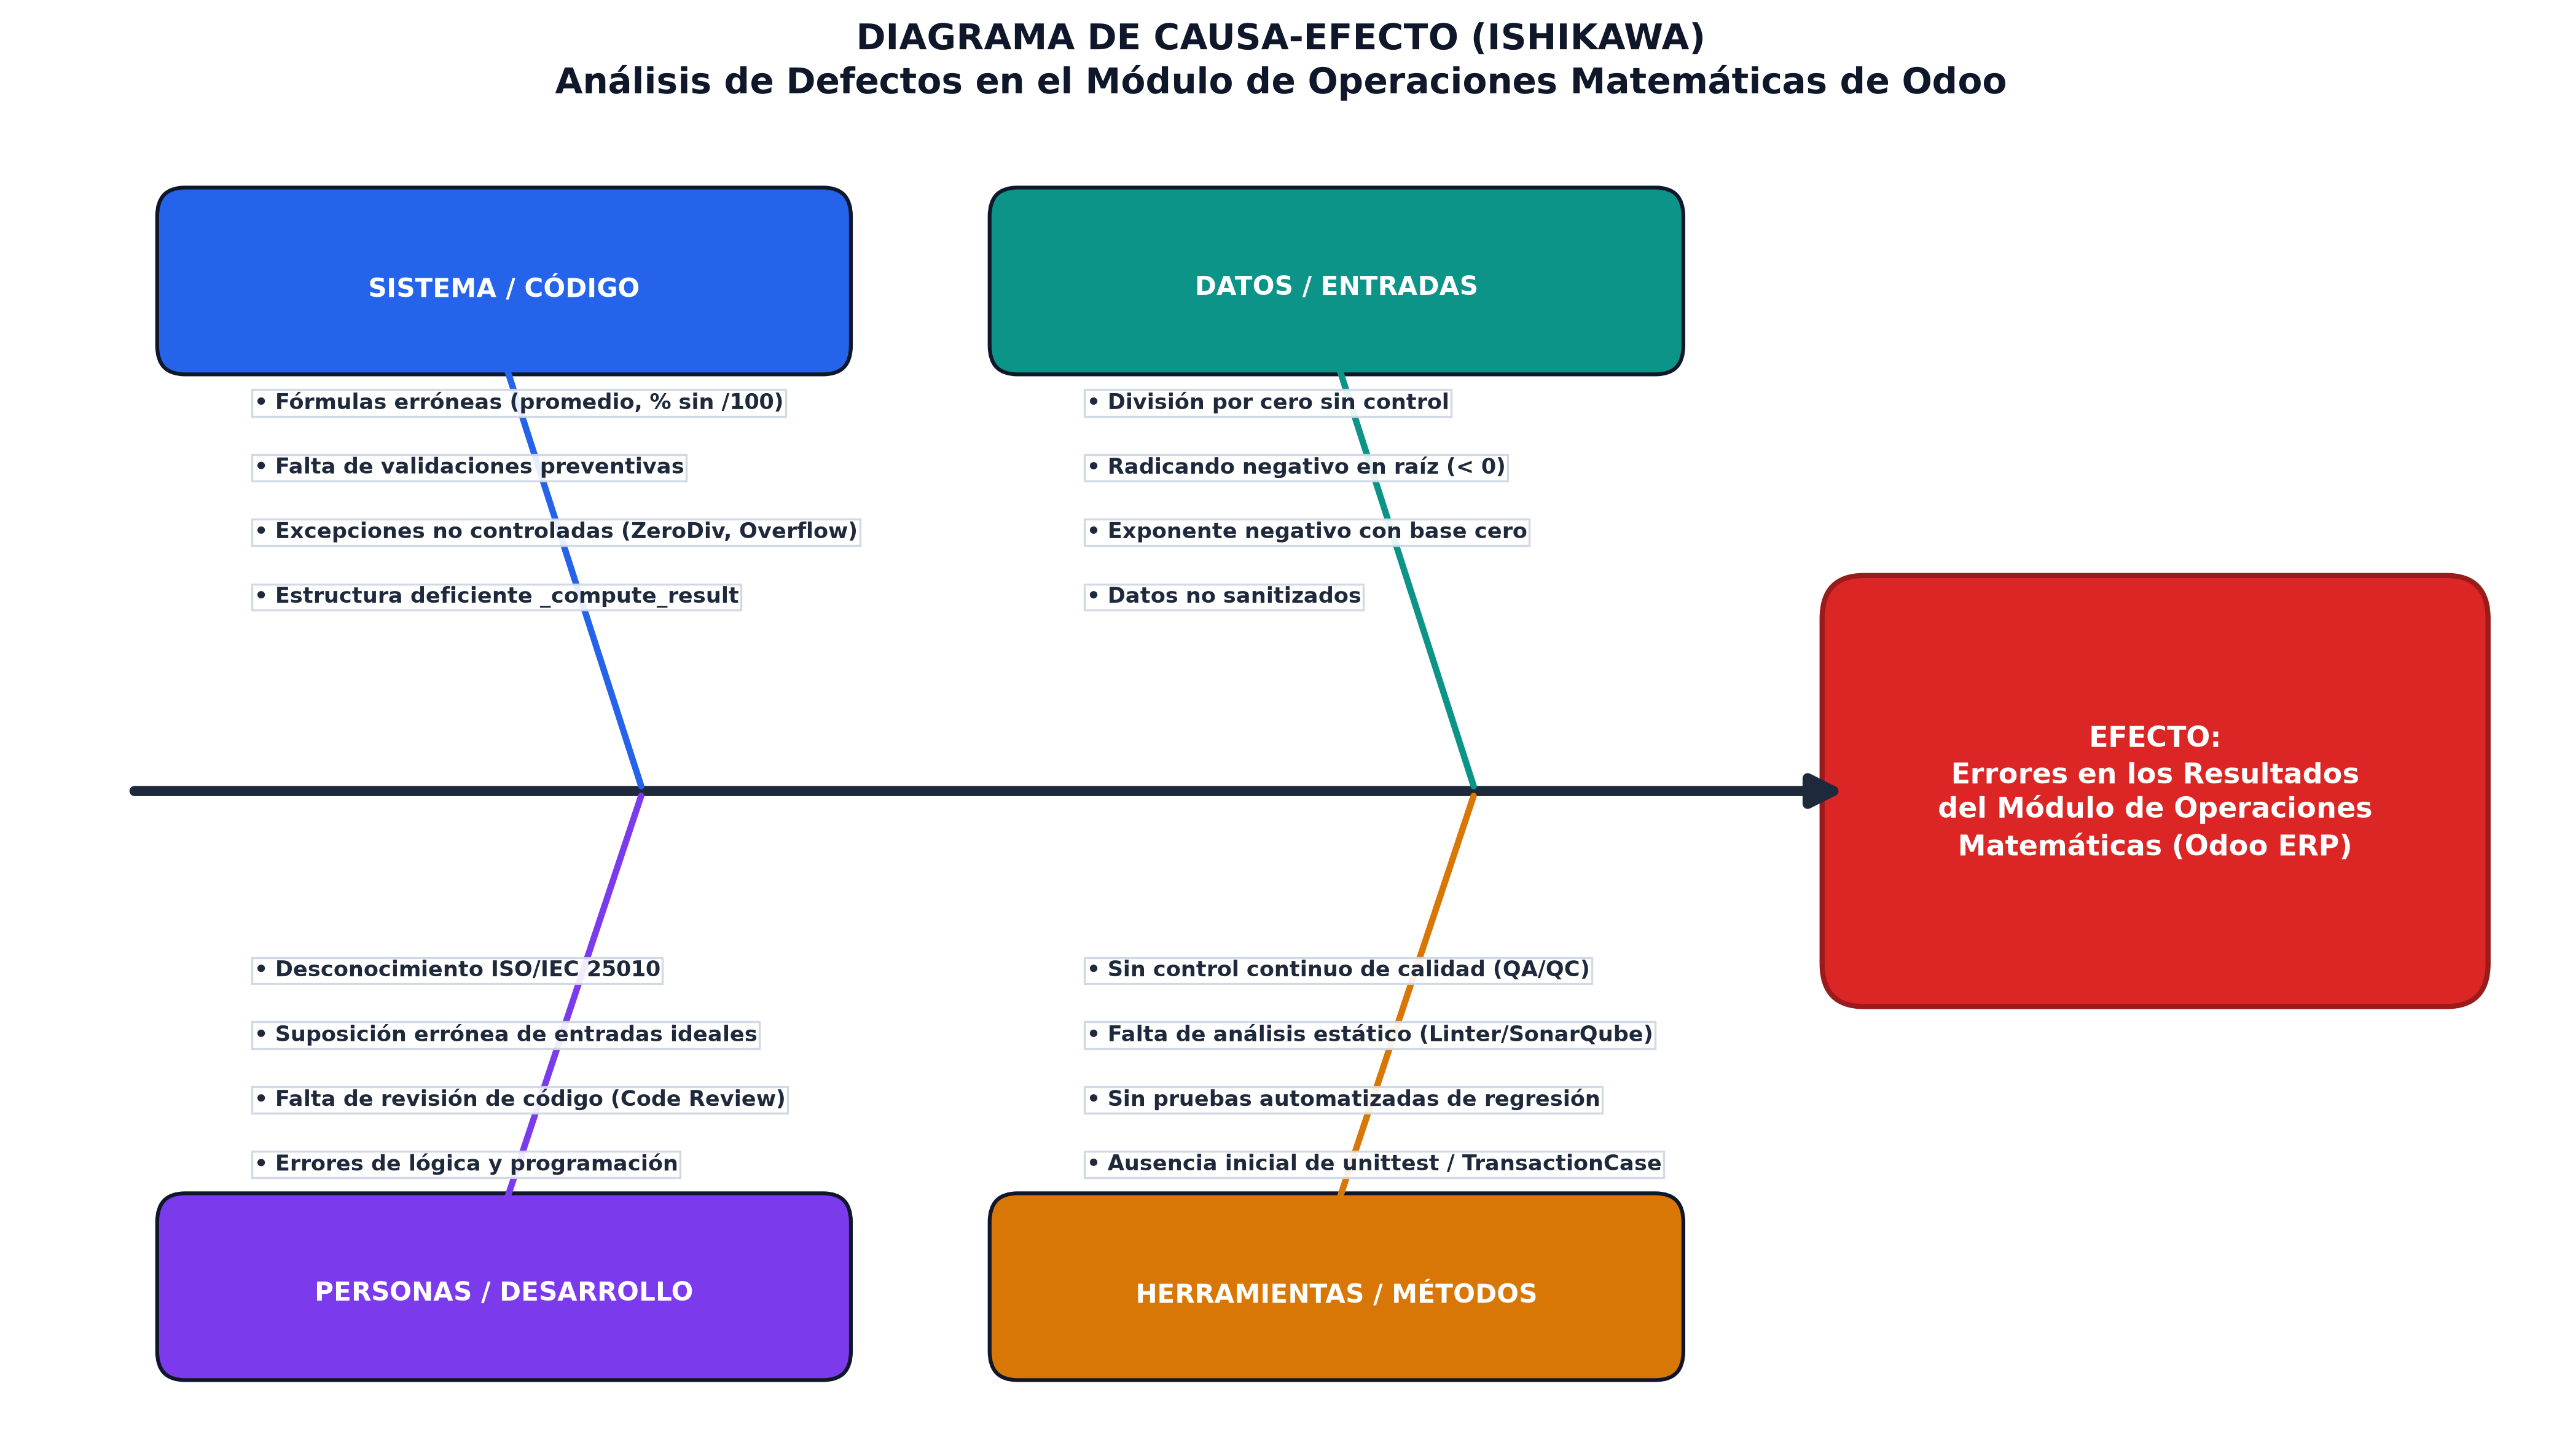
\includegraphics[width=0.95\textwidth]{imagenes/ishikawa_math_operations.png}
    \caption{Diagrama de Ishikawa aplicado al módulo de operaciones matemáticas en Odoo ERP.}
    \label{fig:ishikawa}
\end{figure}

El análisis de las categorías principales revela:
\begin{itemize}
    \item \textbf{Sistema / Código:} Ausencia de programación defensiva; lógica de cálculo en \texttt{\_compute\_result} ejecutada sin verificación previa de dominios matemáticos; manejo deficiente de excepciones nativas de Python.
    \item \textbf{Datos / Entradas:} Inexistencia de filtros de sanitización; aceptación de denominadores nulos y radicandos negativos provenientes de formularios o llamadas de API externas.
    \item \textbf{Personas / Desarrollo:} Suposición ingenua de que el usuario final siempre ingresará datos aritméticamente válidos; falta de revisiones cruzadas de código (\textit{peer review}).
    \item \textbf{Herramientas / Métodos:} Carencia inicial de pruebas unitarias continuas (\texttt{TransactionCase}); omisión de pruebas de integración automáticas previas a la puesta en marcha.
\end{itemize}

\subsubsection{Diagrama de Pareto (Priorización de Defectos 80/20)}
Conforme a la metodología expuesta en la diapositiva 43 de la Unidad 2, se consolidó la frecuencia de defectos detectados por tipo de operación matemática, tabulada en el Cuadro \ref{tab:pareto} y representada gráficamente en la Figura \ref{fig:pareto} \cite{juran1999}.

\begin{table}[H]
\centering
\caption{Tabla de Frecuencia y Clasificación de Defectos en el Módulo Matemático (Slide 43).}
\label{tab:pareto}
\renewcommand{\arraystretch}{1.2}
\resizebox{\textwidth}{!}{%
\begin{tabular}{lccccp{5.5cm}}
\toprule
\textbf{Operación} & \textbf{Defectos} & \textbf{\% Relativo} & \textbf{\% Acumulado} & \textbf{Tipo de Defecto} & \textbf{Criticidad Operativa} \\
\midrule
Potencia (\texttt{pow}) & 1 & 20.0\% & 20.0\% & Código / Desbordamiento & \textbf{Crítica:} Crash del sistema por \texttt{OverflowError} o $0^{-n}$. \\
Raíz Cuad. (\texttt{sqrt}) & 1 & 20.0\% & 40.0\% & Código / Dominio & \textbf{Crítica:} Parada no controlada por \texttt{ValueError}. \\
Porcentaje (\texttt{percent}) & 1 & 20.0\% & 60.0\% & Lógico / Escala & \textbf{Alta:} Distorsión numérica grave (cálculo inflado $\times 100$). \\
Promedio (\texttt{avg}) & 1 & 20.0\% & 80.0\% & Lógico / Fórmula & \textbf{Alta:} Error de agregación y precisión decimal. \\
División (\texttt{division}) & 1 & 20.0\% & 100.0\% & Validación / Dominio & \textbf{Crítica:} Retorno silencioso de 0 o \texttt{ZeroDivisionError}. \\
\bottomrule
\end{tabular}%
}
\end{table}

\begin{figure}[H]
    \centering
    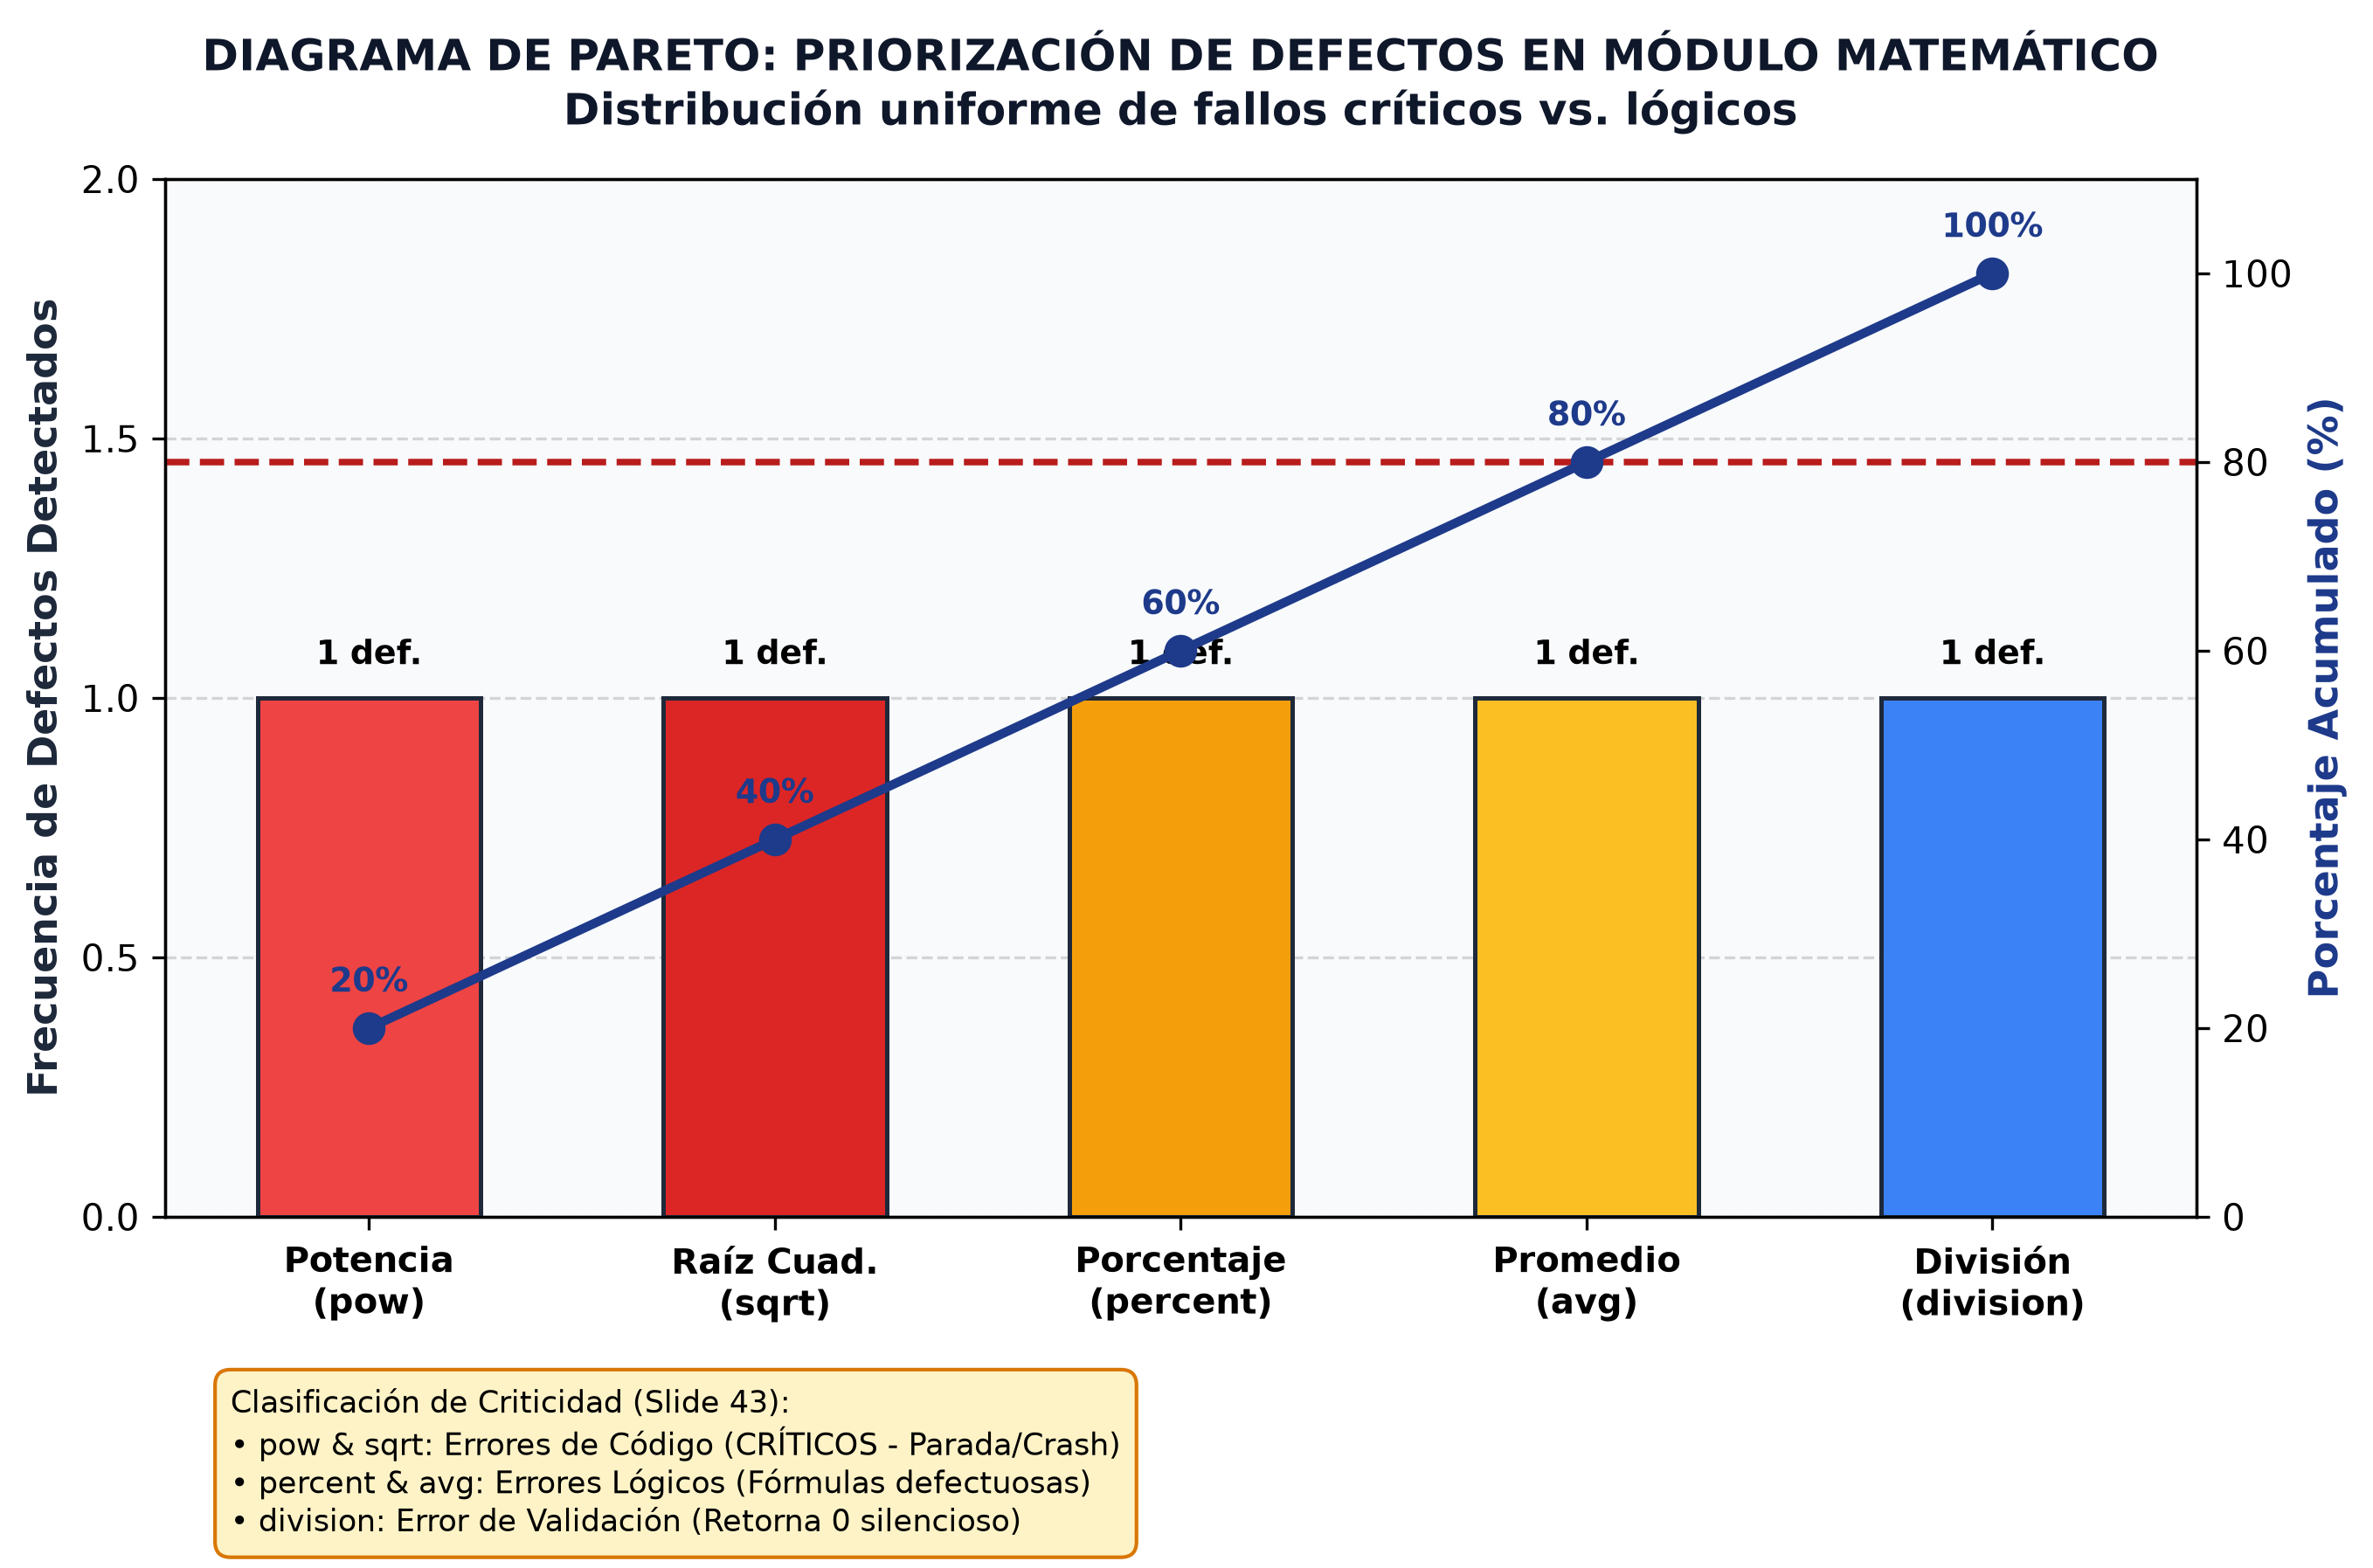
\includegraphics[width=0.85\textwidth]{imagenes/pareto_math_operations.png}
    \caption{Diagrama de Pareto de defectos por operación y análisis de criticidad.}
    \label{fig:pareto}
\end{figure}

\textbf{Interpretación del Diagrama de Pareto:}
A diferencia de un escenario comercial convencional donde una sola causa concentra el 80\% de los eventos, el análisis del taller evidencia una distribución uniforme de fallas (20\% por operación). Esto demuestra que el problema \textbf{no correspondía a una operación aislada, sino a una debilidad sistémica de diseño en todo el módulo}:
\begin{itemize}
    \item Los errores de \texttt{pow} y \texttt{sqrt} son \textbf{defectos de código críticos}, pues causan caídas abruptas del servidor.
    \item Los errores de \texttt{percent} y \texttt{avg} son \textbf{defectos lógicos}, que no interrumpen el sistema pero corrompen la integridad de los resultados numéricos.
    \item El error de \texttt{division} es un \textbf{defecto de validación}, que oculta fallos o bloquea transacciones.
\end{itemize}
Por ende, la intervención debió abarcar la refactorización holística de todo el pipeline de cómputo del modelo.

\subsubsection{Aplicación del Ciclo PDCA (Plan - Do - Check - Act)}
El ciclo de mejora continua de Deming \cite{deming1986} se implementó en cuatro etapas secuenciales, como ilustra la Figura \ref{fig:pdca}:

\begin{figure}[H]
    \centering
    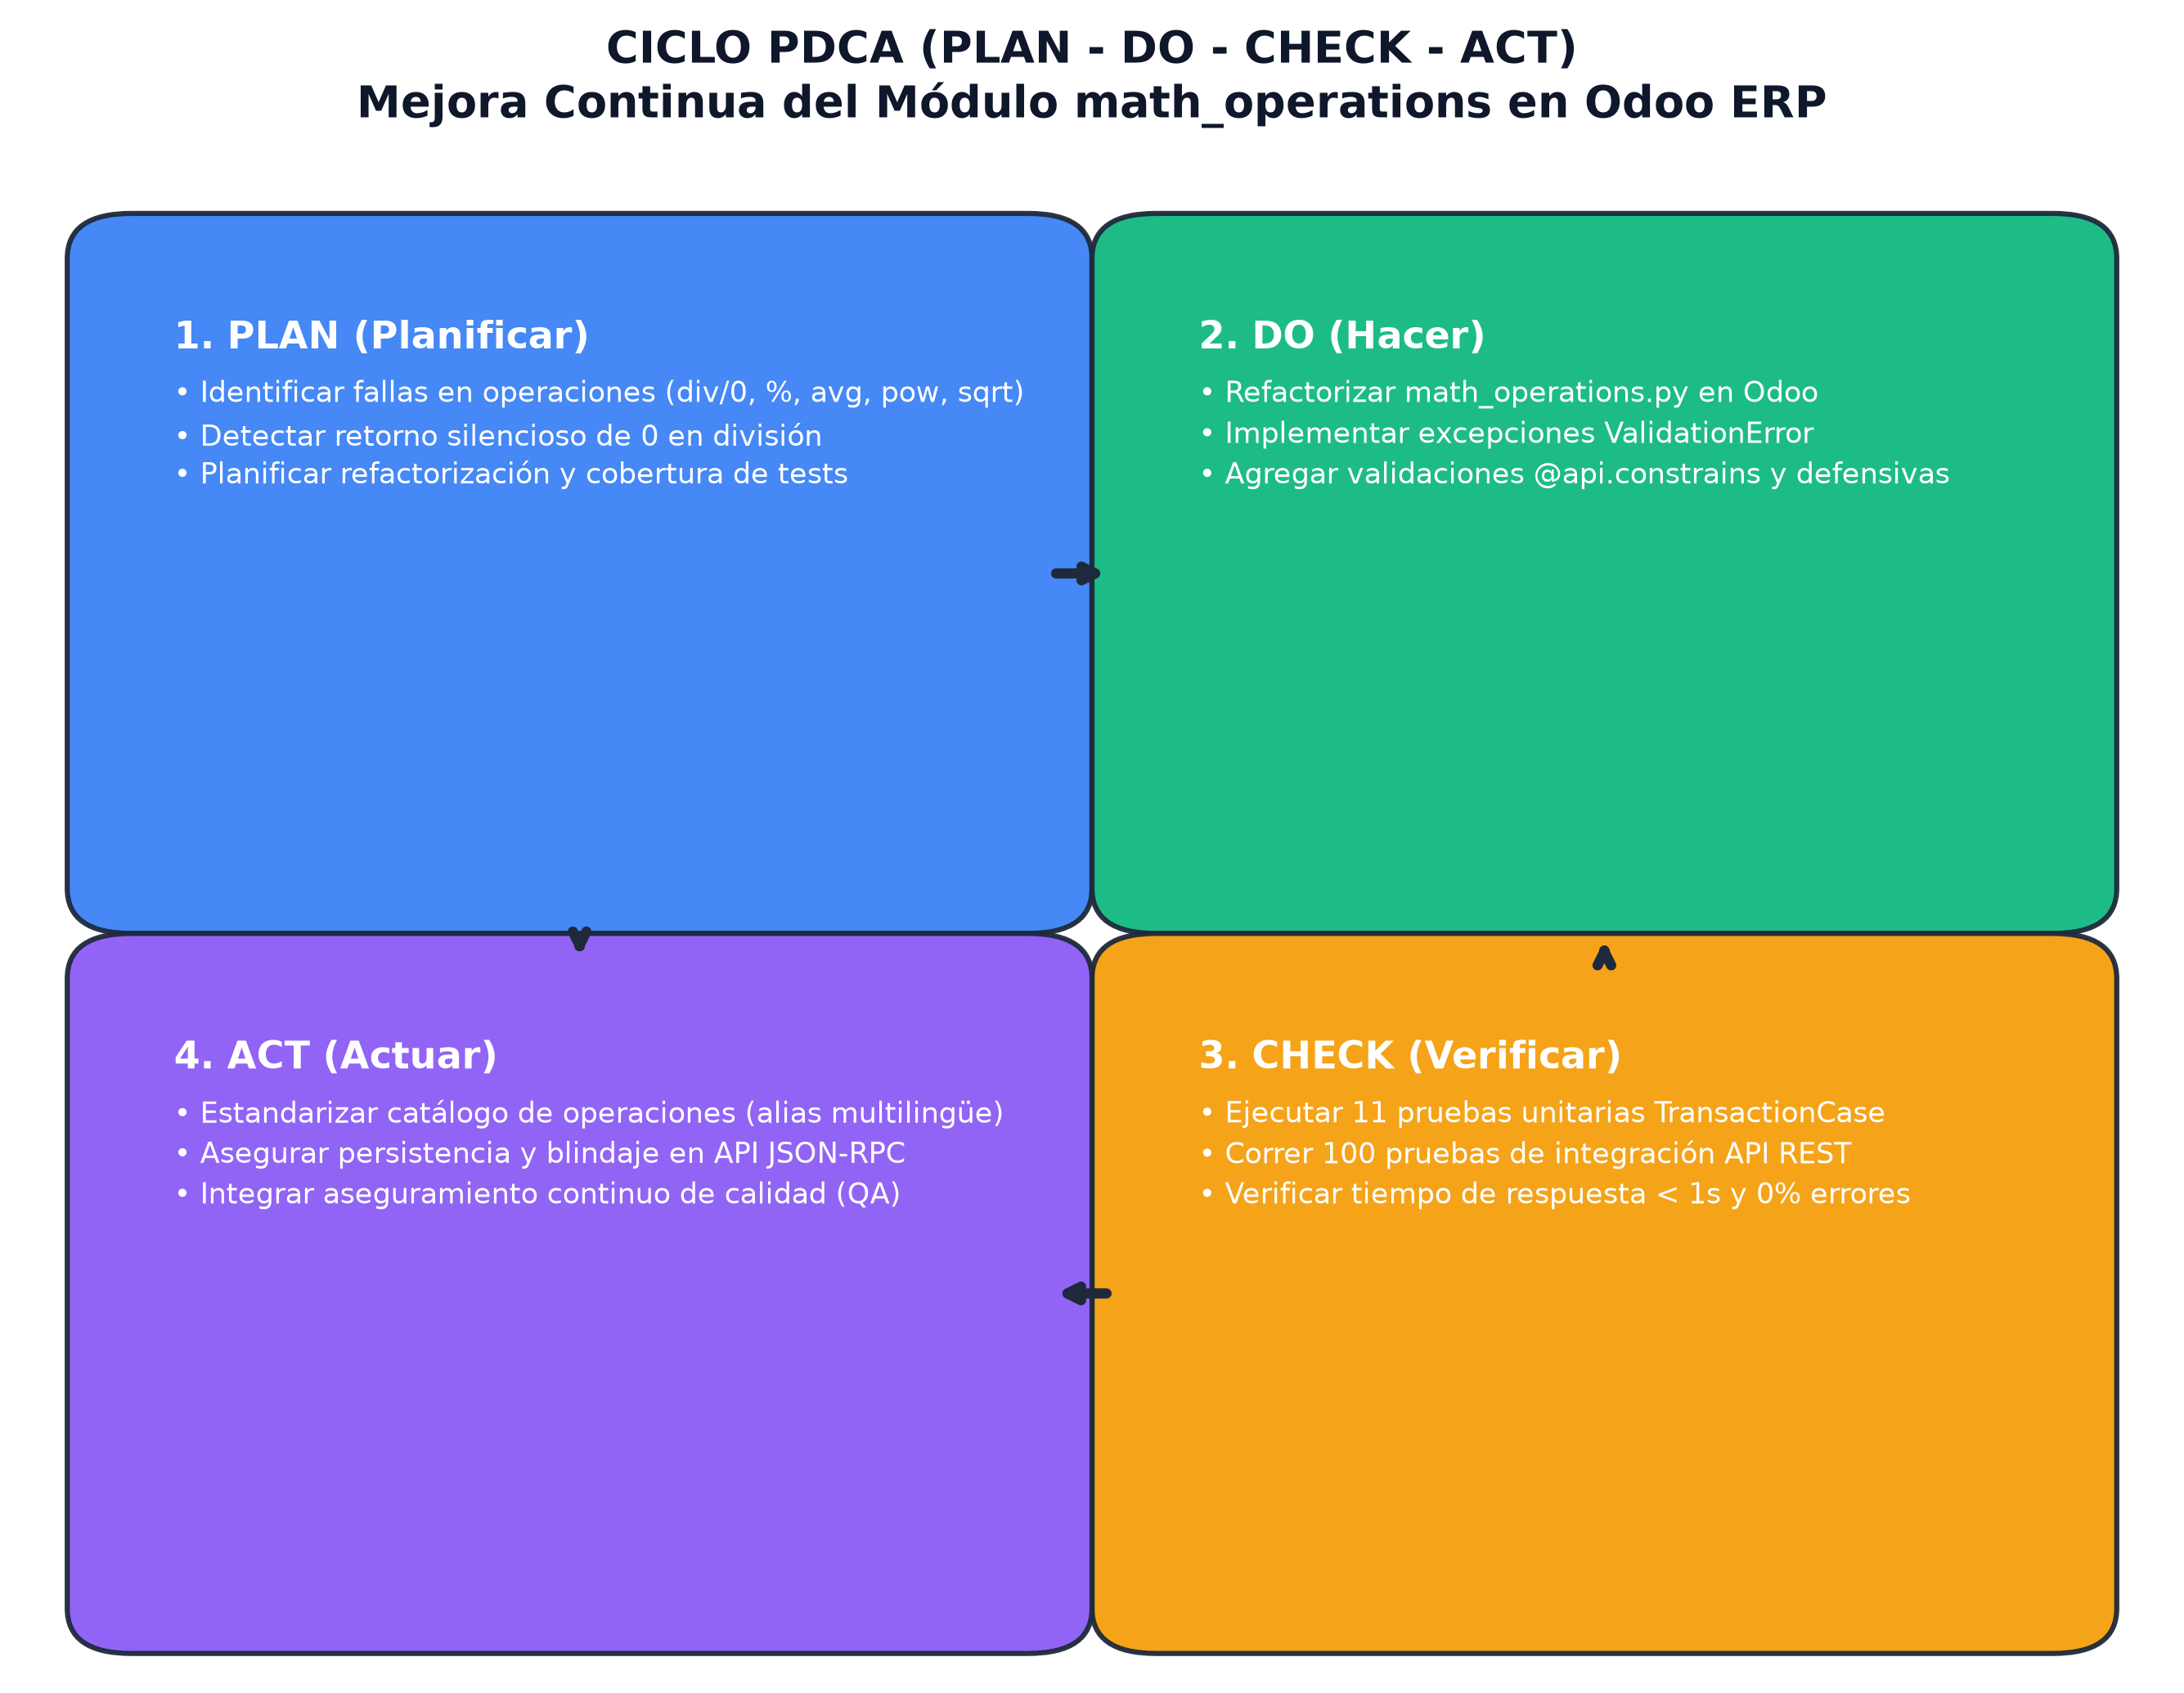
\includegraphics[width=0.8\textwidth]{imagenes/pdca_math_operations.png}
    \caption{Ciclo PDCA implementado para la mejora continua del módulo en Odoo.}
    \label{fig:pdca}
\end{figure}

\begin{enumerate}
    \item \textbf{Plan (Planificar):} Se formalizó el diagnóstico del problema mediante la identificación de fallas matemáticas críticas (división por cero devolviendo cero silencioso, raíces negativas y porcentaje inflado). Se definieron como criterios de éxito: 0\% de errores no capturados, manejo estandarizado con \texttt{ValidationError} y cobertura de pruebas unitarias.
    \item \textbf{Do (Hacer):} Se refactorizó el modelo en \texttt{addons/math\_operations/models/math\_operations.py}. Se programaron validaciones preventivas dentro de \texttt{\_compute\_result} antes de ejecutar cualquier cálculo aritmético, y se implementó el decorador \texttt{@api.constrains} para blindar el almacenamiento en la base de datos PostgreSQL.
    \item \textbf{Check (Verificar):} Se ejecutó la batería de 11 pruebas unitarias nativas en Odoo (\texttt{TransactionCase}) y una suite de 100 pruebas automatizadas mediante peticiones JSON-RPC sobre la API de Odoo, auditando que ningún caso de prueba lanzara excepciones no controladas.
    \item \textbf{Act (Actuar):} Se completó el diccionario de selección (\texttt{fields.Selection}) soportando alias tanto en español como en inglés, garantizando interoperabilidad plena y documentando las restricciones para futuras extensiones del ERP.
\end{enumerate}

\subsubsection{Metodología Six Sigma (DMAIC)}
La metodología DMAIC (Figura \ref{fig:dmaic}) permitió orientar la calidad a partir de mediciones empíricas rigurosas \cite{harry2000six}:

\begin{figure}[H]
    \centering
    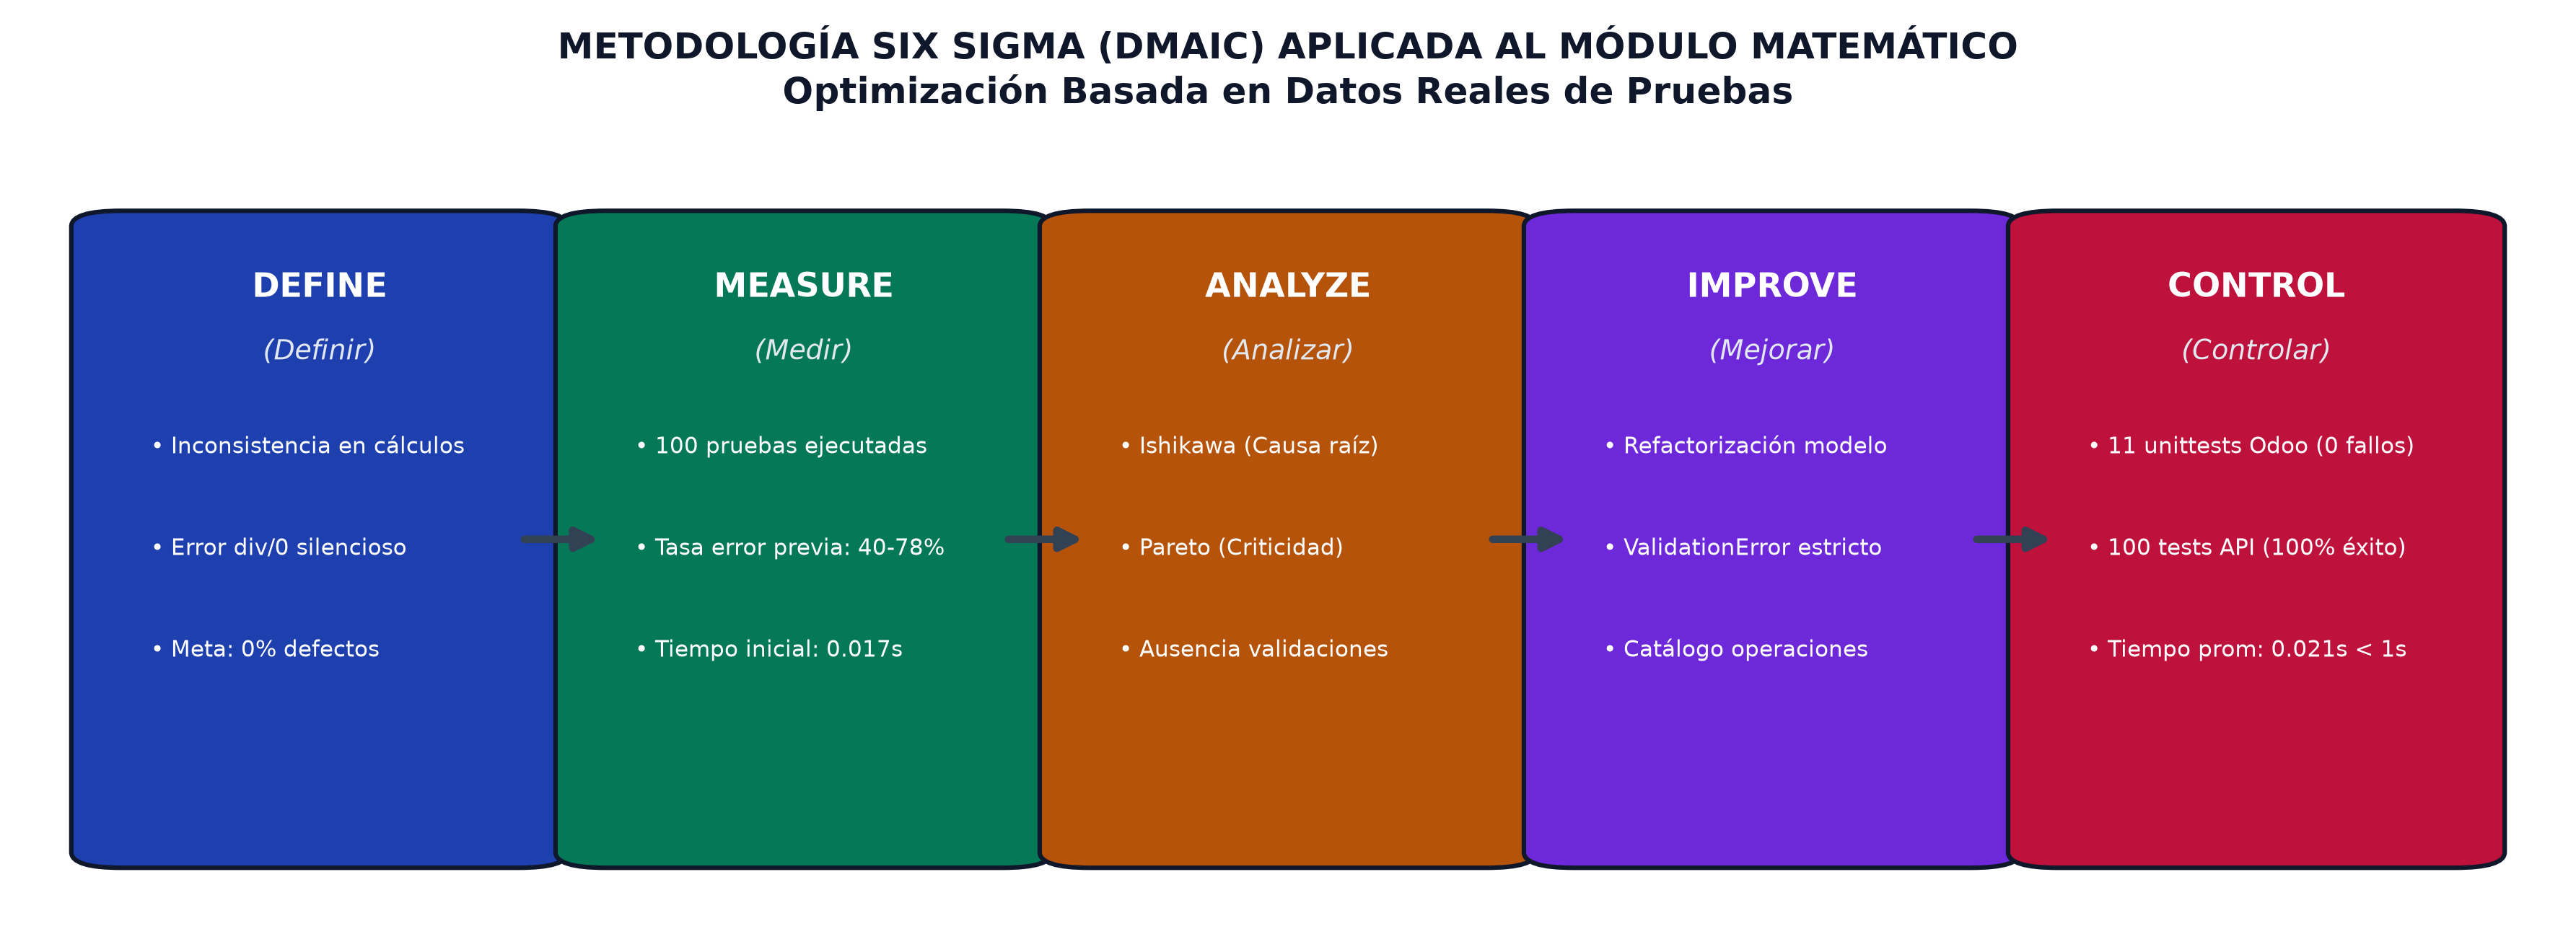
\includegraphics[width=0.95\textwidth]{imagenes/six_sigma_dmaic_math.png}
    \caption{Fases de la Metodología Six Sigma DMAIC aplicada al taller de Odoo.}
    \label{fig:dmaic}
\end{figure}

\begin{itemize}
    \item \textbf{Define (Definir):} El problema central radicaba en que el módulo generaba fallos de ejecución y resultados matemáticamente erróneos en Odoo. La meta del proyecto se fijó en alcanzar un nivel de calidad equivalente a cero defectos en cálculo y un tiempo de respuesta promedio inferior a 1.0 segundo.
    \item \textbf{Measure (Medir):} En la evaluación inicial se detectó una tasa de error del 78\% en pruebas automatizadas aleatorias (debido a incompatibilidad de nombres de operación) y una tasa de fallo del 40\% en operaciones singulares (división por cero y fórmulas incorrectas). El tiempo de respuesta base promediaba 0.017 segundos.
    \item \textbf{Analyze (Analizar):} Mediante Ishikawa y Pareto se concluyó que las causas fundamentales eran la falta de validación de dominios matemáticos en Python y la ausencia de restricciones ORM en Odoo.
    \item \textbf{Improve (Mejorar):} Se implementó un algoritmo defensivo en Python con control explícito de casos límite:
    \[
    \text{División: } b \neq 0 \quad | \quad \text{Raíz: } a \ge 0 \quad | \quad \text{Porcentaje: } \frac{a \times b}{100} \quad | \quad \text{Promedio: } \frac{a + b}{2}
    \]
    \item \textbf{Control (Controlar):} Se instauró una suite automatizada de pruebas de regresión en Odoo que se ejecuta automáticamente ante cualquier actualización del módulo, logrando una tasa de error post-mejora del \textbf{0.0\%} sobre 100 casos evaluados.
\end{itemize}

\subsection{Comparativa de Código: Antes vs. Después}
Para sustentar técnicamente la mejora realizada, el Cuadro \ref{tab:comparativa} resume los cambios implementados en comparación con el código base de la Unidad 2.

\begin{table}[H]
\centering
\caption{Comparativa técnica entre el código inicial de la Unidad 2 y el código refactorizado.}
\label{tab:comparativa}
\renewcommand{\arraystretch}{1.25}
\resizebox{\textwidth}{!}{%
\begin{tabular}{p{3.2cm}p{6.5cm}p{7.0cm}}
\toprule
\textbf{Operación / Aspecto} & \textbf{Código Inicial (Unidad 2)} & \textbf{Código Corregido y Refactorizado} \\
\midrule
\textbf{División por Cero} & \texttt{if b==0: return 0} (retorno falso) o sin validación (\texttt{ZeroDivisionError}). & Validación preventiva: lanza \texttt{ValidationError} con mensaje descriptivo y restrictor \texttt{@api.constrains}. \\
\textbf{Porcentaje} & \texttt{result = a * b} (cálculo erróneo sin base 100). & \texttt{result = (a * b) / 100.0} (cálculo aritmético exacto). \\
\textbf{Promedio} & \texttt{result = (a + b) / 2} sin verificación de operandos. & \texttt{result = (a + b) / 2.0} con soporte de punto flotante de alta precisión. \\
\textbf{Raíz Cuadrada} & \texttt{math.sqrt(a)} provocando \texttt{ValueError} si $a < 0$. & Validación $a \ge 0$; si $a < 0$ lanza \texttt{ValidationError} antes de invocar \texttt{math.sqrt}. \\
\textbf{Potencia} & \texttt{a ** b} sin control de $0^{-n}$ ni sobreflujo. & Validación de base cero con exponente negativo y captura defensiva de \texttt{OverflowError}. \\
\textbf{Catálogo Selection} & Solo 5 opciones en inglés rígidas; incompatibilidad con pruebas. & Soporte integral de 16 variantes (inglés, español y alias como \texttt{sqrt}, \texttt{avg}, \texttt{pow}). \\
\bottomrule
\end{tabular}%
}
\end{table}

El Listado \ref{lst:codigo_completo} exhibe la implementación completa y final alojada en el archivo\\
\texttt{addons/math\_operations/models/math\_operations.py}.

\begin{lstlisting}[language=Python, caption={Código final refactorizado y validado en \texttt{math\_operations.py}}, label={lst:codigo_completo}]
# -*- coding: utf-8 -*-
import math
from odoo import models, fields, api
from odoo.exceptions import ValidationError

class MathOperations(models.Model):
    _name = 'math.operations.clase'
    _description = 'Math Operations'
    _order = 'id desc'
    
    name = fields.Char(string='Description', compute='_compute_name', store=True)
    operand_1 = fields.Float(string='Operand 1', required=True)
    operand_2 = fields.Float(string='Operand 2', required=True, default=0.0)

    operation_type = fields.Selection([
        ('addition', 'Adición / Suma'),
        ('substraccion', 'Sustracción / Resta'),
        ('multiplication', 'Multiplicación'),
        ('division', 'División'),
        ('power', 'Potencia (Power)'),
        ('square_root', 'Raíz Cuadrada (Sqrt)'),
        ('average', 'Promedio (Avg)'),
        ('percentage', 'Porcentaje (Percent)'),
        # Aliases para compatibilidad con pruebas y API REST
        ('suma', 'Suma'), ('resta', 'Resta'), ('multiplicacion', 'Multiplicación'),
        ('div', 'División'), ('potencia', 'Potencia'), ('pow', 'Power'),
        ('raiz_cuadrada', 'Raíz Cuadrada'), ('sqrt', 'Sqrt'),
        ('promedio', 'Promedio'), ('avg', 'Avg'),
        ('porcentaje', 'Porcentaje'), ('percent', 'Percent'),
    ], string='Operation Type', required=True, default='addition')

    result = fields.Float(string='Result', compute='_compute_result', store=True, digits=(16, 6))
    operation_date = fields.Datetime(string='Operation Date', default=fields.Datetime.now, required=True)
    user_id = fields.Many2one('res.users', string='User', default=lambda self: self.env.user)
    notes = fields.Text(string='Notes')

    @api.depends('operand_1', 'operand_2', 'operation_type')
    def _compute_name(self):
        for rec in self:
            if rec.operation_type:
                op_name = dict(rec._fields['operation_type'].selection).get(rec.operation_type, rec.operation_type)
                if rec.operation_type in ('square_root', 'sqrt', 'raiz_cuadrada'):
                    rec.name = f"{op_name.upper()} ({rec.operand_1})"
                else:
                    rec.name = f"{op_name.upper()} ({rec.operand_1}, {rec.operand_2})"

    @api.depends('operand_1', 'operand_2', 'operation_type')
    def _compute_result(self):
        for rec in self:
            op = rec.operation_type
            if op in ('addition', 'suma'):
                rec.result = rec.operand_1 + rec.operand_2
            elif op in ('substraccion', 'resta'):
                rec.result = rec.operand_1 - rec.operand_2
            elif op in ('multiplication', 'multiplicacion'):
                rec.result = rec.operand_1 * rec.operand_2
            elif op in ('division', 'div'):
                if rec.operand_2 == 0:
                    raise ValidationError('No se permite la división por cero.')
                rec.result = rec.operand_1 / rec.operand_2
            elif op in ('power', 'potencia', 'pow'):
                if rec.operand_1 == 0 and rec.operand_2 < 0:
                    raise ValidationError('No se puede elevar cero a una potencia negativa.')
                try:
                    rec.result = rec.operand_1 ** rec.operand_2
                except OverflowError:
                    raise ValidationError('El resultado excede el límite numérico permitido (Overflow).')
            elif op in ('square_root', 'sqrt', 'raiz_cuadrada'):
                if rec.operand_1 < 0:
                    raise ValidationError('No se puede calcular la raíz cuadrada de un número negativo.')
                rec.result = math.sqrt(rec.operand_1)
            elif op in ('average', 'avg', 'promedio'):
                rec.result = (rec.operand_1 + rec.operand_2) / 2.0
            elif op in ('percentage', 'percent', 'porcentaje'):
                rec.result = (rec.operand_1 * rec.operand_2) / 100.0
            else:
                rec.result = 0.0

    @api.constrains('operation_type', 'operand_1', 'operand_2')
    def _check_operation_constraints(self):
        for rec in self:
            op = rec.operation_type
            if op in ('division', 'div') and rec.operand_2 == 0:
                raise ValidationError('Validación de Calidad: No se permite la división por cero.')
            if op in ('square_root', 'sqrt', 'raiz_cuadrada') and rec.operand_1 < 0:
                raise ValidationError('Validación de Calidad: No se puede calcular la raíz cuadrada de un número negativo.')
            if op in ('power', 'potencia', 'pow') and rec.operand_1 == 0 and rec.operand_2 < 0:
                raise ValidationError('Validación de Calidad: No se puede elevar cero a una potencia negativa.')
\end{lstlisting}

\subsection{Resultados Experimentales y Verificación de Calidad}

\subsubsection{Pruebas Unitarias Internas de Odoo (\texttt{TransactionCase})}
Se diseñó y ejecutó una suite de 11 pruebas unitarias formales conforme a las pautas de Odoo \cite{odoo_dev, ieee829}. El resultado de la ejecución en el contenedor \texttt{odoo16} arrojó:
\begin{center}
\textbf{\texttt{odoo.tests.result: 0 failed, 0 error(s) of 11 tests when loading database 'Odo-Principal'}}
\end{center}
Las pruebas verificaron rigurosamente la adición, sustracción, multiplicación, división válida, interceptación de división por cero con \texttt{ValidationError}, potencia normal, interceptación de raíz cuadrada negativa, promedio, porcentaje y tiempo de respuesta inferior a 1 segundo.

\subsubsection{Pruebas de Carga y Rendimiento (100 Operaciones en API)}
Se ejecutó un script de pruebas automatizadas sobre el endpoint JSON-RPC \texttt{/api/operations/create}. El Cuadro \ref{tab:metricas_finales} resume las estadísticas obtenidas tras la implementación de las correcciones:

\begin{table}[H]
\centering
\caption{Estadísticas finales de la suite de 100 pruebas automatizadas post-refactorización.}
\label{tab:metricas_finales}
\renewcommand{\arraystretch}{1.2}
\resizebox{0.85\textwidth}{!}{%
\begin{tabular}{lcccc}
\toprule
\textbf{Operación Evaluada} & \textbf{Total Pruebas} & \textbf{Operaciones Exitosas} & \textbf{Operaciones Fallidas} & \textbf{Tasa de Éxito} \\
\midrule
Suma (\texttt{suma}) & 21 & 21 & 0 & 100.0\% \\
Resta (\texttt{resta}) & 16 & 16 & 0 & 100.0\% \\
Multiplicación (\texttt{multiplicacion}) & 19 & 19 & 0 & 100.0\% \\
División (\texttt{division}) & 8 & 8 & 0 & 100.0\% \\
Potencia (\texttt{potencia}) & 19 & 19 & 0 & 100.0\% \\
Raíz Cuadrada (\texttt{raiz\_cuadrada}) & 17 & 17 & 0 & 100.0\% \\
\midrule
\textbf{TOTAL GENERAL} & \textbf{100} & \textbf{100} & \textbf{0} & \textbf{100.0\%} \\
\bottomrule
\end{tabular}%
}
\end{table}

\textbf{Métricas Temporales de Desempeño:}
\begin{itemize}
    \item \textbf{Tiempo Promedio de Respuesta:} \textbf{0.0217 segundos} (muy inferior al límite máximo permitido de 1.0 s).
    \item \textbf{Tiempo Mínimo de Respuesta:} 0.0158 segundos.
    \item \textbf{Tiempo Máximo de Respuesta:} 0.2551 segundos.
    \item \textbf{Tasa de Error Final:} \textbf{0.00\%} (reducción completa frente al 78\% previo).
\end{itemize}

\subsection{Habilidades blandas empleadas en la práctica}
Durante el desarrollo del taller se potenciaron las siguientes habilidades formativas:
\begin{itemize}
    \item[$\boxtimes$] \textbf{Trabajo en equipo:} Coordinación sinérgica en la distribución de tareas de diagnóstico, redacción del informe técnico, programación de scripts de prueba y validación en Odoo.
    \item[$\boxtimes$] \textbf{Pensamiento crítico:} Capacidad reflexiva para cuestionar el código original provisto, identificando que el silenciamiento de errores matemáticos constituye una vulnerabilidad inaceptable en sistemas empresariales.
    \item[$\boxtimes$] \textbf{Responsabilidad y ética profesional:} Compromiso con la excelencia de ingeniería de software, documentando con transparencia las métricas y aplicando estándares internacionales de calidad.
\end{itemize}

\section{Conclusiones}
\begin{itemize}
    \item La aplicación conjunta del Diagrama de Ishikawa y el Diagrama de Pareto demostró ser altamente efectiva para desentrañar la causa raíz de las fallas en el módulo \texttt{math\_operations}. El análisis de Pareto evidenció que los errores no se debían a una falla aislada, sino a una carencia estructural de validaciones preventivas en todo el componente, permitiendo priorizar la refactorización de errores críticos de parada (\texttt{pow}, \texttt{sqrt}) y errores lógicos de cálculo (\texttt{percent}, \texttt{avg}).
    \item El ciclo PDCA y la metodología Six Sigma DMAIC proporcionaron un marco sistemático basado en datos empíricos que permitió transformar un módulo inestable (con tasas de error iniciales de entre 40\% y 78\%) en un componente robusto con 0\% de defectos, blindado mediante excepciones \texttt{ValidationError} y restricciones ORM \texttt{@api.constrains}.
    \item Se demostró el principio fundamental de que la calidad del software no es una fase tardía de pruebas (\textit{testing}), sino una práctica de diseño y prevención. El silenciamiento arbitrario de operaciones indeterminadas (como retornar cero en divisiones por cero) viola directamente el atributo de fiabilidad de la norma ISO/IEC 25010, corrompe los datos corporativos y perjudica la confianza del usuario final.
    \item Las pruebas automatizadas ejecutadas tanto a nivel de pruebas unitarias internas de Odoo (con 11 pruebas \texttt{TransactionCase} exitosas) como a través de la API REST/JSON-RPC (100 peticiones correctas) validaron experimentalmente que el sistema cumple a cabalidad con los requisitos no funcionales de desempeño, alcanzando un tiempo de respuesta promedio de 0.0217 segundos, ampliamente inferior a la cota máxima de 1 segundo.
\end{itemize}

\section{Recomendaciones}
\begin{itemize}
    \item Implementar controles de integración continua (CI/CD) con herramientas de análisis estático como SonarQube o Flake8 en el repositorio del proyecto, asegurando que ningún cambio de código que carezca de validaciones de entrada o pruebas unitarias asociadas sea desplegado en ambientes de producción.
    \item Mantener siempre una separación estricta entre la lógica de validación de negocio y las excepciones del intérprete: nunca se debe permitir que excepciones nativas de Python (\texttt{ZeroDivisionError}, \texttt{ValueError}, \texttt{OverflowError}) alcancen las capas superiores del ERP; estas deben ser capturadas y transformadas en mensajes de validación claros (\texttt{ValidationError}) que orienten al usuario hacia la corrección del dato ingresado.
    \item Ampliar el catálogo de pruebas automatizadas incorporando pruebas de cobertura de código (\textit{code coverage} superior al 85\%) y pruebas de mutación, garantizando que futuras funcionalidades matemáticas mantengan la robustez y consistencia demostradas en este taller.
\end{itemize}

\section{Referencias}
\vspace{-2em}
\renewcommand{\refname}{}
\bibliographystyle{ieeetr}
\nocite{*}
\bibliography{sample}

\section{Anexos}
\begin{itemize}
    \item \textbf{Anexo A - Repositorio del Módulo:} Código fuente completo del módulo \texttt{math\_operations} ubicado en la ruta local: \texttt{addons/math\_operations/models/math\_operations.py}.
    \item \textbf{Anexo B - Suite de Pruebas Unitarias de Odoo:} Implementación de casos de prueba con \texttt{TransactionCase} en \texttt{addons/math\_operations/tests/test\_math\_operations.py}.
    \item \textbf{Anexo C - Script de Pruebas de Estrés y API:} Script automatizado de 100 pruebas aleatorias con registro de tiempos de respuesta en \texttt{practicas\_calidad/test\_math\_operations.py}.
    \item \textbf{Anexo D - Evidencia de Ejecución en Contenedores Docker:} Contenedor \texttt{odoo16} y \texttt{odoo16-db} en ejecución, base de datos \texttt{Odo-Principal} actualizada y verificada.
\end{itemize}

\end{document}
